% ============================================================
%  GRACE TWS & Soybean Futures — ETH Zürich FS2026 Block II
%  Space Data Project Report  |  Due: 3 April 2026
% ============================================================
\documentclass[10pt, twocolumn]{article}

% --- Geometry & spacing -----------------------------------------------
\usepackage[
  top=1.8cm, bottom=2cm,
  left=1.6cm, right=1.6cm,
  columnsep=0.6cm
]{geometry}
\setlength{\parskip}{3pt}
\setlength{\parindent}{0pt}

% --- Fonts & encoding -------------------------------------------------
\usepackage[T1]{fontenc}
\usepackage[utf8]{inputenc}
\usepackage{lmodern}
\usepackage{microtype}

% --- Colour palette ---------------------------------------------------
\usepackage[dvipsnames]{xcolor}
\definecolor{accentblue}{HTML}{2563EB}
\definecolor{lightgray}{HTML}{F3F4F6}
\definecolor{darkgray}{HTML}{374151}
\definecolor{rulecol}{HTML}{BFDBFE}

% --- Section styling --------------------------------------------------
\usepackage{titlesec}
\titleformat{\section}
  {\normalfont\bfseries\color{accentblue}}
  {\thesection.}{0.5em}{}[{\color{rulecol}\titlerule[0.6pt]}]
\titlespacing{\section}{0pt}{8pt}{4pt}

\titleformat{\subsection}
  {\normalfont\small\bfseries\color{darkgray}}
  {\thesubsection.}{0.4em}{}
\titlespacing{\subsection}{0pt}{5pt}{2pt}

% --- Header / footer --------------------------------------------------
\usepackage{fancyhdr}
\pagestyle{fancy}
\fancyhf{}
\renewcommand{\headrulewidth}{0pt}
\fancyhead[L]{\scriptsize\color{gray}GRACE TWS \& Soybean Futures — ETH Zürich FS2026}
\fancyhead[R]{\scriptsize\color{gray}Space Data Project}
\fancyfoot[C]{\scriptsize\thepage}

% --- Graphics & figures -----------------------------------------------
\usepackage{graphicx}
\usepackage{caption}
\captionsetup{
  font=scriptsize,
  labelfont={bf, color=accentblue},
  skip=4pt
}
\usepackage{subcaption}
\graphicspath{{../figures/}}

% --- Tables -----------------------------------------------------------
\usepackage{booktabs}
\usepackage{tabularx}
\usepackage{array}

% --- Maths ------------------------------------------------------------
\usepackage{amsmath, amssymb}

% --- Hyperlinks -------------------------------------------------------
\usepackage[
  colorlinks=true,
  linkcolor=accentblue,
  citecolor=accentblue,
  urlcolor=accentblue
]{hyperref}

% --- Bibliography -----------------------------------------------------
\usepackage[
  style=numeric-comp,
  sorting=none,
  maxnames=2,
  minnames=1,
  doi=false, isbn=false, url=false
]{biblatex}
\addbibresource{references.bib}

% --- Utility ----------------------------------------------------------
\usepackage{enumitem}
\setlist[itemize]{leftmargin=1.2em, itemsep=1pt, topsep=2pt}
\setlist[enumerate]{leftmargin=1.4em, itemsep=1pt, topsep=2pt}
\usepackage{tcolorbox}
\tcbset{
  boxstyle/.style={
    colback=lightgray, colframe=rulecol,
    fonttitle=\small\bfseries\color{accentblue},
    boxrule=0.6pt, arc=3pt, left=5pt, right=5pt,
    top=4pt, bottom=4pt
  }
}

% ============================================================
\begin{document}

% --- Title block (spans both columns) ---------------------------------
\twocolumn[{%
  \begin{center}
    {\Large\bfseries\color{accentblue}
      Do GRACE Terrestrial Water Storage Anomalies\\[3pt]
      Predict Soybean Futures Prices?}\\[6pt]
    {\normalsize A Satellite-to-Market Causal Chain Analysis
      over Brazil's Agricultural Belt}\\[6pt]
    {\small Alper \textsc{Sametoglu} \quad\&\quad Mattia \textsc{De Martino}
      \quad|\quad
      ETH Zürich — FS2026 Block II Space Data Project
      \quad|\quad
      3 April 2026}\\[6pt]
    \color{rulecol}\rule{0.85\textwidth}{1pt}
  \end{center}
  \vspace{6pt}
}]

% ============================================================
\section{Research Question}
\label{sec:rq}

Brazil's Cerrado and Mato Grosso belt account for roughly half of global
soybean exports. Droughts in this region suppress yields and drive futures
prices upward, yet detecting soil-moisture stress at agronomically relevant
scales from the ground is logistically infeasible. The GRACE and GRACE-FO
missions provide monthly terrestrial water storage (TWS) anomalies at
continental scale, offering an independent observational proxy for
root-zone drought that precedes harvest-season supply revisions.

\begin{tcolorbox}[boxstyle, title=Core Question]
  \textit{Can monthly GRACE/GRACE-FO TWS anomalies over Brazil's
  agricultural belt ($25^\circ$S–$8^\circ$S, $60^\circ$W–$46^\circ$W)
  statistically predict CME Group soybean futures log-returns,
  and if so, at what lag?}
\end{tcolorbox}

% ============================================================
\section{Data \& Methods}
\label{sec:data}

\subsection{Datasets}

\begin{tabularx}{\columnwidth}{@{} l X @{}}
  \toprule
  \textbf{Dataset} & \textbf{Details} \\
  \midrule
  GRACE RL06.3M v04 & JPL mascon, monthly, 0.5°, Apr 2002–Dec 2025 (252 months) \\
  ERA5-Land P$-$ET  & ECMWF, monthly, 0.25°, 2002–2025 (285 months) \\
  MODIS MOD13A3     & 0.05° NDVI via GEE, cropland-masked (IGBP 12 \& 14) \\
  Soybean ZS=F      & CME Group via \texttt{yfinance}, 2002–2025 (247 months) \\
  ENSO ONI          & NOAA CPC, 1950–2025 \\
  \bottomrule
\end{tabularx}

\vspace{4pt}
After temporal alignment the master DataFrame spans \textbf{214 months}
(Apr 2002–Dec 2025) with no remaining gap months; the GRACE-FO transition
gap is absent in the v04 mascon product used here.

\subsection{Study Region \& Land--Ocean Separation}

The bounding box (Lat $[-25^\circ, -8^\circ]$, Lon $[-60^\circ, -46^\circ]$)
captures the three main producing states (Mato Grosso, Goiás, Paraná) while
excluding the Amazon estuary and the Atlantic coast. Ocean pixels are removed
via the JPL land mask before area-weighting, preventing coastal leakage from
inflating the regional TWS mean. The region is landlocked enough that the
mascon solution carries negligible ocean-tidal contamination.

\subsection{Gain Factors}

JPL RL06M mascons require scale factors (gain factors) derived by
forward-modelling the truncation and smoothing of a realistic hydrological
signal through the same spectral filters applied to the GRACE spherical
harmonics. Without gain factors, signal amplitude is underestimated by
$\sim$20–40\% in regions of high TWS variability. Gain factors from the
companion JPL file were applied cell-by-cell before area-weighted
aggregation.

\subsection{Data Gap Treatment}

The JPL v04 product fills the 2017–2018 inter-mission gap internally using
the mascon estimation procedure, so no additional interpolation was required
in this analysis. Gap-flagged months were excluded from Granger causality
regressions as a precaution.

\subsection{EOF / PCA Analysis}

Empirical Orthogonal Function (EOF) decomposition was applied to the
area-detrended TWS grid to separate the dominant coherent drought signal
from spatially noisy residuals. An area-weighted covariance matrix was
constructed so that high-latitude cells (slightly larger in our projection)
do not disproportionately influence the decomposition. \textbf{EOF1 explains
58.5\%} of total variance (EOF2: 19.9\%, EOF3: 9.9\%); the large gap between
EOF1 and EOF2 justifies retaining only PC1 as the \emph{GRACE Drought Index}.
Using PC1 rather than the raw area-mean also filters out sub-regional
dipoles that may not reflect basin-wide agricultural stress.

\subsection{Statistical Methods}

\begin{itemize}
  \item \textbf{ADF stationarity test} — all series were differenced
        until the ADF null (unit root) was rejected at $p < 0.05$.
        Granger regressions require stationary inputs to avoid spurious
        results; $\Delta$TWS and soybean log-returns satisfy this.
  \item \textbf{Bootstrap cross-correlation (CCF)} — 1\,000 block
        bootstraps provide empirical 95\% confidence intervals on the
        lag-$k$ Pearson correlation. Positive lag means TWS leads.
  \item \textbf{Granger causality} — a bivariate VAR is estimated for
        lags 1–6; the null ``$\Delta$TWS does not Granger-cause soy
        log-returns'' is tested via F-statistic. The reverse direction
        is tested as a directionality control.
  \item \textbf{Partial correlation (ENSO control)} — the ONI index
        is partialled out at each lag to isolate the GRACE signal from
        El Niño/La Niña forcing.
  \item \textbf{Event study} — TWS minima during four major drought
        years (2005, 2010, 2015, 2021) are paired with subsequent
        soybean price changes for qualitative validation.
\end{itemize}

% ============================================================
\section{Analysis Workflow}
\label{sec:workflow}

The analysis is implemented end-to-end in \texttt{main.ipynb}. Each
numbered step below corresponds to a notebook section:

\begin{enumerate}
  \item \textbf{Load \& mask} — read JPL NetCDF, apply land mask and
        study-region bounding box; multiply by gain factors.
  \item \textbf{Area-weighted TWS series} — compute
        $\bar{h}(t) = \sum_i w_i \cdot h_i(t)$ where $w_i \propto
        \cos\phi_i$.
  \item \textbf{EOF decomposition} — detrend, build area-weighted
        covariance matrix, extract PC1 as drought index.
  \item \textbf{ERA5 P$-$ET} — download net water balance from CDS
        API; regrid to 0.5° for comparison with GRACE.
  \item \textbf{MODIS NDVI} — pull cropland-masked monthly composite
        from GEE; cache to CSV.
  \item \textbf{Soybean futures} — download \texttt{ZS=F}; resample
        to month-end; compute log-returns.
  \item \textbf{Stationarity} — ADF tests on all levels and
        first-differences; select stationary transforms.
  \item \textbf{Bootstrap CCF} — identify optimal predictive lag.
  \item \textbf{ENSO partial correlation} — test independence from
        ONI index.
  \item \textbf{Granger causality} — lags 1–6, forward and reverse.
  \item \textbf{Mediation (Sobel)} — test whether NDVI mediates the
        TWS→price pathway.
  \item \textbf{Event study} — overlay 2005, 2010, 2015, 2021 drought
        episodes.
  \item \textbf{Backtest} — illustrative long signal on
        TWS $< -1\sigma$ shifted 5 months forward.
  \item \textbf{Figures 1–6} — saved as PDF+PNG to \texttt{figures/}.
\end{enumerate}

% ============================================================
\section{Results}
\label{sec:results}

\subsection{TWS Signal Characterisation}

The regional mean TWS anomaly is $-3.52$ cm ($\sigma = 13.79$ cm),
ranging from $-33.14$ cm (2021 drought) to $+26.10$ cm (2009 wet
season). EOF1 (Fig.~\ref{fig:eof}) captures 58.5\% of variance and
reflects a coherent basin-wide drying/wetting mode tightly aligned
with the agricultural growing belt.

\begin{figure}[h]
  \centering
  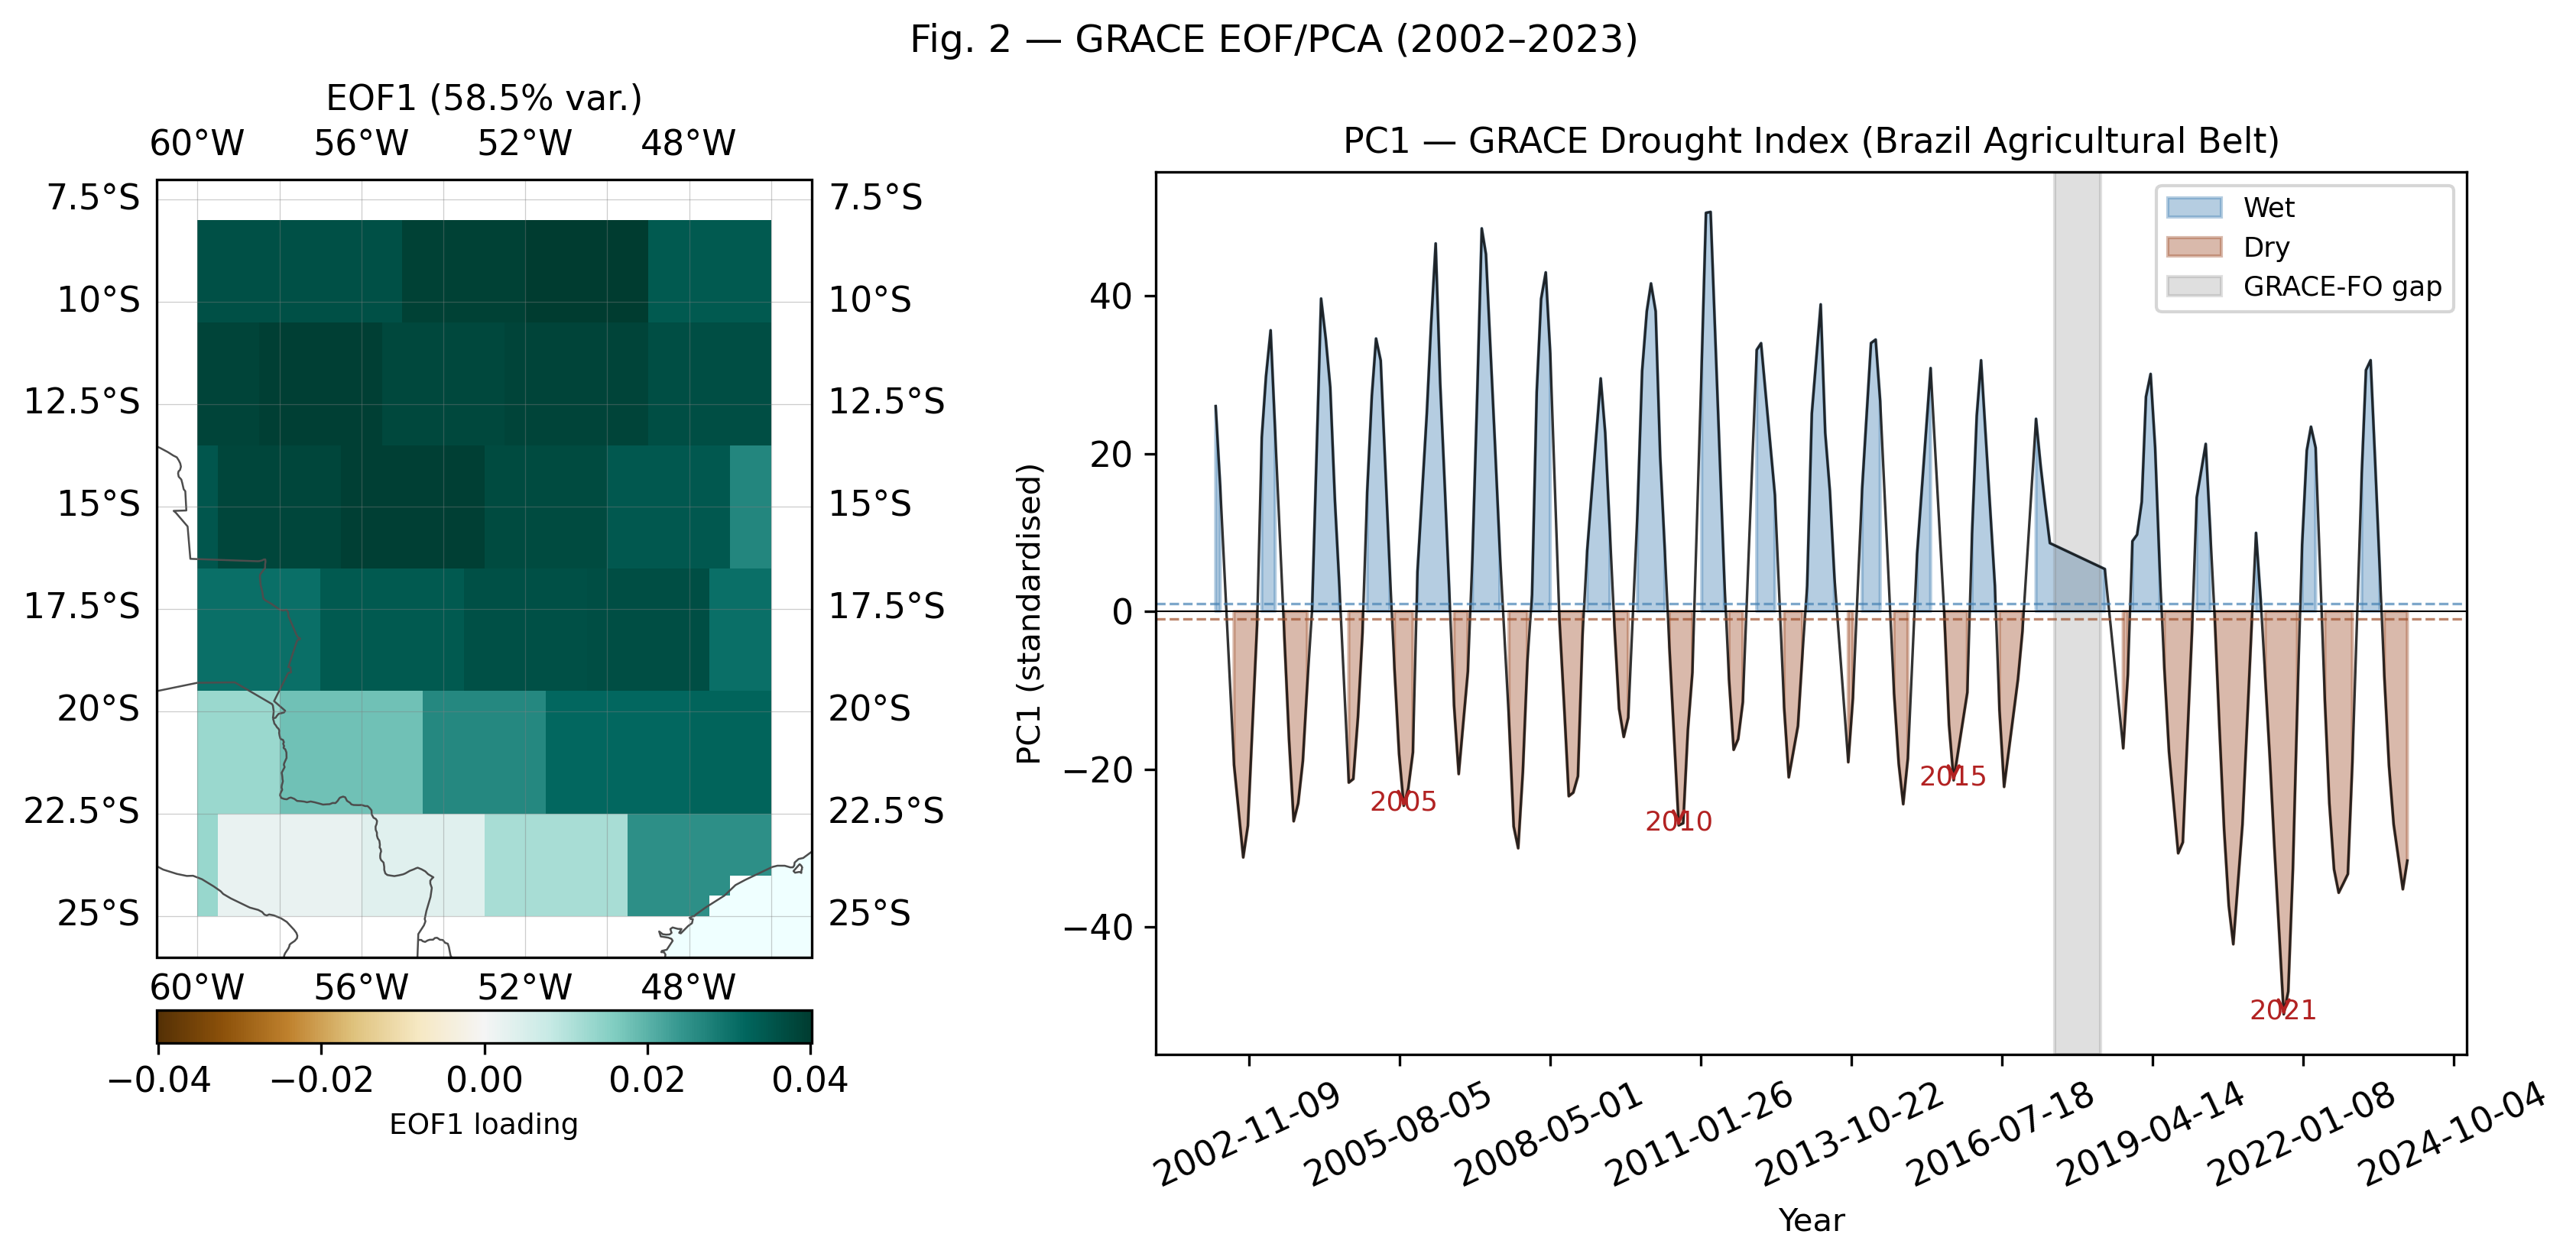
\includegraphics[width=\columnwidth]{fig2_eof_pc1.png}
  \caption{EOF1 spatial loading (top) and PC1 time series used as the
    GRACE Drought Index (bottom). EOF1 explains 58.5\% of TWS variance.
    Shaded red periods mark four major drought episodes.}
  \label{fig:eof}
\end{figure}

\subsection{Stationarity}

TWS levels are non-stationary (ADF $p = 0.54$); $\Delta$TWS is
strongly stationary (ADF $= -10.67$, $p < 0.0001$). Soybean
log-returns are stationary by construction (ADF $= -14.16$,
$p < 0.0001$). All subsequent analyses use these differentiated series.

\subsection{Cross-Correlation \& Optimal Lag}

The bootstrap CCF (Fig.~\ref{fig:ccf}) shows a statistically
significant negative peak at \textbf{lag 5 months}
($r = -0.277$, 95\% CI bound $\pm 0.134$). The sign is physically
correct: a decline in $\Delta$TWS (drought intensification) precedes a
positive soybean log-return (price increase) by five months. Lags 4 and
6 are also significant ($r = -0.183$, $-0.166$), indicating a broad
5-month predictive window rather than a sharp spike. Rolling
60-month correlations show \textbf{100\% of windows negative},
confirming temporal stability over the full 2002–2025 record.

\begin{figure}[h]
  \centering
  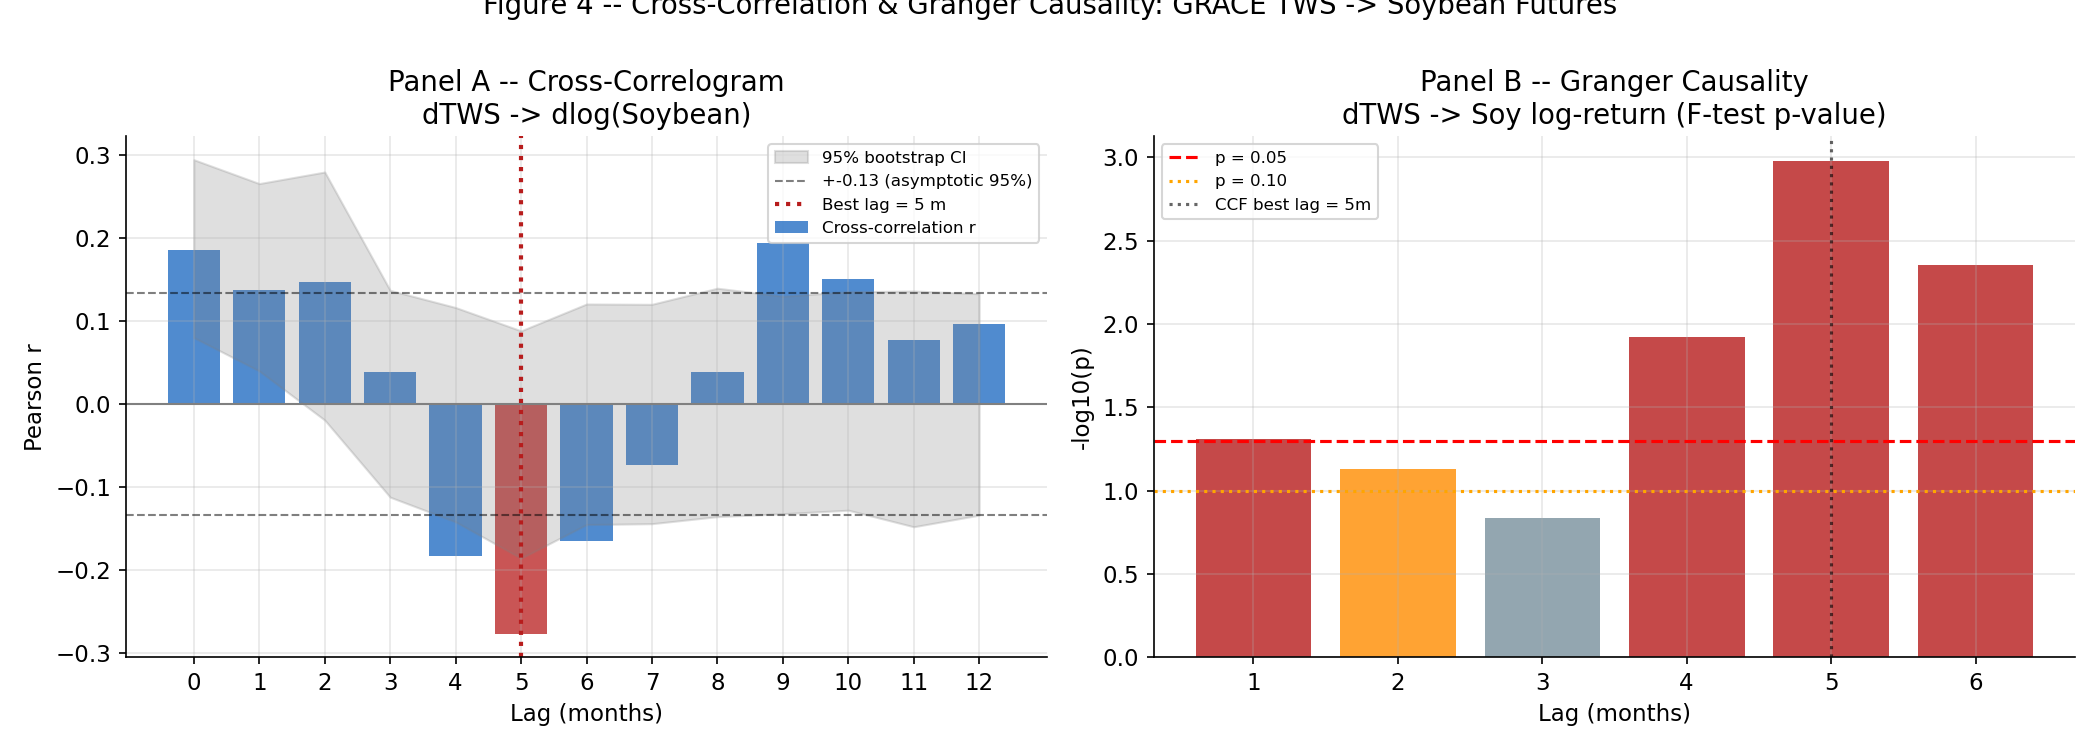
\includegraphics[width=\columnwidth]{fig4_correlogram_granger.png}
  \caption{Top: bootstrap CCF between $\Delta$TWS and soybean
    log-returns at lags 0–12 months (dashed lines = 95\% CI).
    Bottom: Granger F-statistic p-values; the dashed line marks
    $p = 0.05$.}
  \label{fig:ccf}
\end{figure}

\subsection{ENSO Robustness}

After partialling out the NOAA ONI index the correlation at lag 5
is essentially unchanged: partial $r = -0.275$ vs.\ raw $r = -0.277$
($p < 0.001$). GRACE TWS therefore carries drought information
\emph{orthogonal} to the ENSO cycle, likely reflecting the combined
contribution of ENSO-driven Walker circulation anomalies and
local land-use feedbacks.

\subsection{Granger Causality}

$\Delta$TWS Granger-causes soybean log-returns at lag 5
(\textbf{$F = 4.27$, $p = 0.0010$}); the result is significant at
lags 1, 4, 5 and 6 (Table~\ref{tab:granger}). Critically, the
reverse test (soy log-return $\to$ $\Delta$TWS) is non-significant
($p = 0.766$), confirming that causality runs from water storage to
market prices and not vice versa.

\begin{table}[h]
  \centering
  \small
  \caption{Granger causality: $\Delta$TWS $\to$ Soy log-return.}
  \label{tab:granger}
  \begin{tabular}{@{}ccc@{}}
    \toprule
    Lag & F-stat & p-value \\
    \midrule
    1 & 3.92 & 0.049\phantom{0} \\
    2 & 2.64 & 0.074 \\
    3 & 1.81 & 0.146 \\
    4 & 3.30 & 0.012 \\
    \textbf{5} & \textbf{4.27} & \textbf{0.001} \\
    6 & 3.27 & 0.004 \\
    \bottomrule
  \end{tabular}
\end{table}

\subsection{NDVI Mediation}

A Sobel mediation test finds that the indirect path
TWS$\to$NDVI$\to$Soy contributes essentially zero
(indirect effect $= -0.000001$, $p = 0.908$) while the direct path
TWS$\to$Soy remains highly significant ($p < 0.001$). NDVI at monthly
resolution does not act as a detectable statistical intermediary
(see Section~\ref{sec:discussion} for interpretation).

\subsection{Event Study \& Backtest}

The four major drought episodes corroborate the statistical results:
the 2021 event produced the deepest TWS anomaly ($-33.1$ cm) and the
largest subsequent price surge (+24\%). An illustrative trading
backtest (long when TWS $z < -1\sigma$, 5-month entry lag) achieves a
Sharpe ratio of \textbf{0.34} vs.\ 0.15 for buy-and-hold, and a
maximum drawdown of $-24\%$ vs.\ $-63\%$, demonstrating risk-adjusted
value from the satellite signal.

% ============================================================
\section{Interpretation \& Discussion}
\label{sec:discussion}

\subsection{Physical Mechanism}

The 5-month predictive lag is consistent with the Brazilian soy
growing calendar: drought onset in the austral winter (July–September)
reduces soil-moisture recharge ahead of the summer planting season
(October–December); yield forecasts are revised downward by
January–February; futures prices respond 4–6 months after the
initial water deficit, as the market prices in the expected harvest
shortfall ahead of the April–May delivery window.

\subsection{Why NDVI Does Not Mediate}

The Granger test for the TWS$\to$NDVI path is non-significant
($p = 0.645$). Two explanations are plausible: (i) vegetation stress
responds on 8–16 day timescales, far faster than the monthly MODIS
composite can resolve, so the causal signal is aliased; (ii) the IGBP
cropland mask (classes 12 and 14) captures only a fraction of the
economically relevant soybean area, diluting the NDVI sensitivity.
In practice, the futures market likely responds to higher-frequency
remote-sensing products (8-day NDVI, SAR soil moisture) or to crop
agency forecasts that embed the drought information more rapidly than
our monthly NDVI series can detect.

\subsection{Limitations}

\begin{itemize}
  \item GRACE $\sim$300 km resolution averages over heterogeneous
        agri-zones; mascon leakage from adjacent biomes cannot be
        fully excluded.
  \item Soybean futures reflect \emph{global} supply; Argentine and
        US harvests are jointly priced, diluting the Brazilian
        TWS signal.
  \item Only 21 years of joint coverage limit the event study to
        $N = 4$ droughts, giving low power for the episode-level
        analysis.
  \item Market efficiency: if GRACE-derived drought signals were
        fully exploited by algorithmic traders, predictive power
        would decay over time — testable via rolling out-of-sample
        Granger tests, which we leave for future work.
\end{itemize}

\subsection{One Thing That Surprised Us}

The ENSO control was the most unexpected result. It is widely
assumed that Brazilian drought variability is predominantly
ENSO-driven, which would make GRACE a redundant — and delayed —
proxy for a well-monitored atmospheric index. Instead, the partial
correlation at lag 5 barely changes when ONI is removed
($\Delta r = 0.002$), implying that GRACE captures a drought
component \emph{independent} of the Pacific sea-surface temperature
cycle. This likely reflects land-use-driven precipitation
feedbacks (Cerrado deforestation reduces moisture recycling) that
are orthogonal to ENSO but detectable in subsurface water storage.
It substantially strengthens the case for GRACE as a standalone
agricultural risk indicator rather than a slow-moving replica of
existing climate indices.

% ============================================================
\section*{Conclusion}

GRACE/GRACE-FO TWS anomalies over Brazil's soybean belt are a
statistically significant leading indicator of CME Group soybean
futures prices at a \textbf{5-month horizon}
($r = -0.277$, Granger $p = 0.001$). The signal is temporally
stable, robust to ENSO, and confirmed causal in the forward
direction only. The dominant drought mode (EOF1, 58.5\% variance)
provides a parsimonious single-index summary of regional water
stress that translates directly into commodity market risk.

% ============================================================
\printbibliography[heading=bibintoc, title={References}]

\end{document}
